\chapter{Data Pre Processing}
The data usually have a lot of quality issues due to thing like noise
or outliers, missing values or duplicate data. One would like to have
a clean data set to work with, but this is not always the case.  The
The action to perform to \textit{prepare} the data is called the
\textbf{data cleaning}

\section{Similarity and Dissimilarity}
\begin{boxH}
  We can define the \textbf{similarity}, or \textbf{dissimilarity},
  between two data object as a numerical measure of how alike or
  different they are.
\end{boxH}
One of the most common similarity measure is the \textbf{distance} 
between two objects, and there are a lot of different distance
measures.

\subsection{Euclidean Distance}
The \textbf{euclidean distance} is the simplest one, which can be
defined as the square root of the sum of the squared differences
between the two objects. It is defined as:
\begin{equation}
  d(x,y) = \sqrt{\sum\limits_{k=1}^n (x_k - y_k)^2 }
\end{equation}
where $x$ and $y$ are two objects, and $x_k$ and $y_k$ are the $k$-th
attributes of the two objects.

Standardizing of the data may be needed to avoid that some attributes
dominate the distance measure.

\subsection{Minkowsky Distance}
\textbf{Minkowsky distance} is a generalization of Euclidean Distance,
and it is defined as:

\begin{equation}
  d(x,y) = (\sum\limits_{k=1}^n | x_k - y_k |^r )^{1/r} 
\end{equation}
where $r$ is a parameter that can be set to 1, 2 or $\infty$.
If $r=1$ we have the \textbf{Manhattan} distance, if $r=2$ we have the 
\textbf{Euclidean} distance, and if $r=\infty$ we have the 
\textbf{Chebyshev} distance.

\subsection{Mahalanobis Distance}
\textbf{Mahalanobis distance} measures the distance between two points
with respect to a probability distribution with covariance matrix $S$
and also  is thus unit less, scale-invariant, and takes into account
the correlations of the data set. It is defined as:
\begin{equation}
  d(x,y,S) = \sqrt{(x-y)^T S^{-1} (x-y)}
\end{equation}

\section{Data pre-processing tasks}
Data pre-processing has many different tasks that have to be carried
out in order to have a clean data set to work with. We will go over
the main ones.
\subsection{Data aggregation}
\begin{boxH}
  \textbf{Data aggregation }is the process of \textbf{combining} two
  or more \textbf{attributes}(or objects) into a single attribute(or
  object).
\end{boxH}
This is done for three main reasons:
\begin{itemize}
  \item To reduce the number of attributes or objects(Data reduction)
  \item To change the scale of the data, for example from daily to
    monthly
  \item To \textit{stabilize} the data, for example by taking the
    average of the data to reduce the variance
\end{itemize}
Here's an example of data aggregation:
\begin{figure}[H]
  \centering
  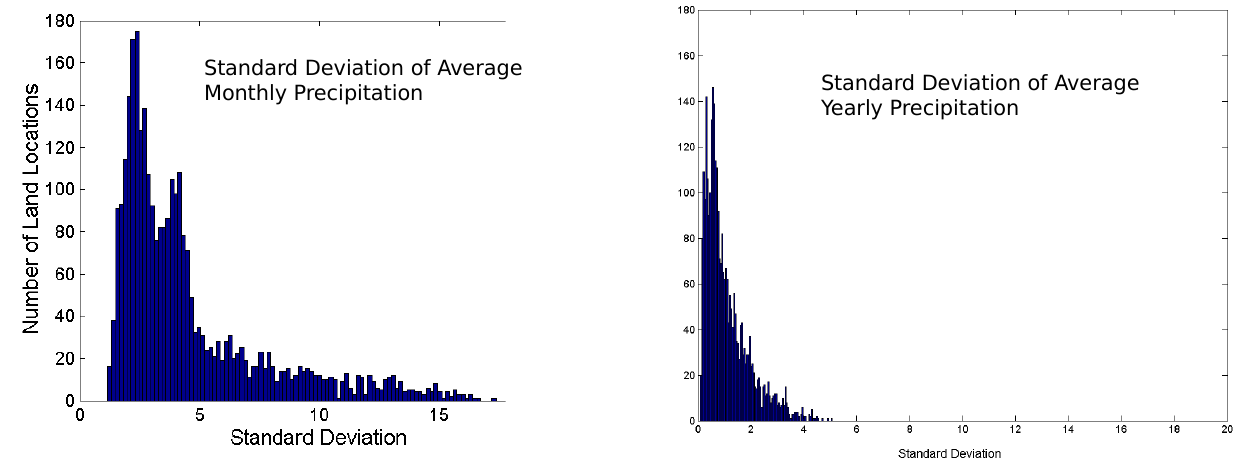
\includegraphics[scale=0.4]{images/Data
  pre-process/precipitation aggregation.png}
  \caption{Example of data aggregation}
  \label{fig:data-aggregation}
\end{figure}
as you can see from figure \ref{fig:data-aggregation}, the yearly
precipitation has much less variability then the average monthly
one.
\subsection{Data reduction}
The main goal of data reduction is to generate a reduced
representation of the dataset, with a much smaller volume but 
still able to produce the same or similar analytical results.\\
This can be done trough different techniques.
\subsubsection{Sampling}
\textbf{Sampling} is the \textbf{main technique} employed for data selection
and it is often used for both the preliminary investigation of the
data and the final data analysis because processing the entire set of
data of interest might be too expensive or time consuming.\\
The key principle for effective sampling is the following: a good
sample will always work like the dataset and can approximately have
the same property.\\
There are several types of sampling like the simple random sampling or
the stratified one that split the data into several partition and then
draw samples from each partition.

\begin{figure}[H]
  \centering
  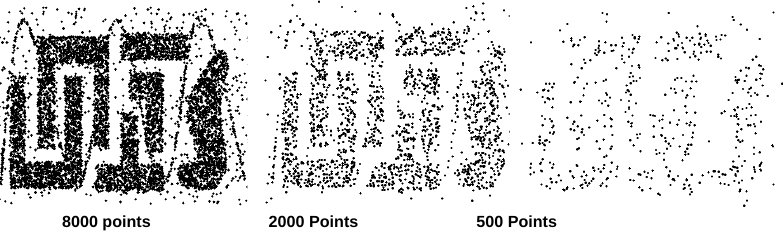
\includegraphics[scale=0.5]{images/Data
  pre-process/sampling.png}
  \caption{Example of sampling}
  \label{fig:sampling}
\end{figure}
There are two main types of sampling:
\begin{itemize}
  \item \textbf{Simple random sampling}: each object has the same probability
    of being selected. Of this type two main methods are: 
    \begin{itemize}
      \item \textbf{With replacement}: the same object can be selected
        more than once because its not removed from the population
      \item \textbf{Without replacement}: the same object can be selected
        only once because it is removed from the population
    \end{itemize}
  \item \textbf{Stratified sampling}: the population is divided into
    subpopulations, and the right number of objects is sampled from
    each subpopulation
\end{itemize}

\subsubsection{Curse of Dimensionality}
When feature dimensionality increases, data becomes increasingly
sparse in the space that it occupies and the definitions of density
and distance between points, which is critical for clustering and
outlier detection, become less meaningful.\\
This is the \textbf{curse of dimensionality}, and it is a common 
problem in data mining and machine learning.
\subsubsection{Feature Subset Selection}
This is another way to reduce the dimensionality of the data, and it
is the process of identifying and removing as much of the irrelevant 
and redundant information as possible.\\
A feature is considered \textbf{irrelevant} if it does not hold any
useful information for the data mining task at hand, while a feature
is considered \textbf{redundant} if it holds the same information as 
another feature.
\subsubsection{Recursive feature elimination}
One method is called recursive feature elimination that assigns
weights to features and then selects features by recursively 
considering smaller and smaller sets of features.  First, the 
estimator is trained on the initial set of features and the 
importance of each feature is obtained, the least important features 
are pruned from current set of features. That procedure is 
recursively repeated on the pruned set until the desired number of 
features to select is eventually reached.
\section{Feature Engineering}
\begin{boxH}
  A \textbf{feature} is an individual measurable property or
  characteristic of the raw data. \textbf{Feature engineering} is the 
  act of extracting features from raw data and transforming them to 
  more useful, from a lot to few.
\end{boxH}
Usually formats that are suitable for machine learning are used.
According to the type of data under analysis different feature
engineering techniques are needed:
\begin{itemize}
  \item \textbf{structured data}: data that can be easily organized
    into a table format, like a spreadsheet
  \item \textbf{unstructured data}: data that does not have a 
    pre-defined format, like text
\end{itemize}
There are many diffrent techniques for feature engineering, like
normalization, discretization, binarization, and many others.

\subsection{Data Transformation}
\textbf{Data transformation} is the process of converting data from
one format to another and it is useful because non numerical data is
difficult to analyze if not transformed into numerical and to capture
important information or to better visualize the data

\subsection{Discretization}
\textbf{Discretization }is the process of converting a continuous
attribute into an ordinal attribute: A potentially infinite number of
values are mapped into a small number of categories, for example
{high, medium, low} or binary attributes or one-hot encoding. 

\subsection{Binarization}
\textbf{Binarization} is the process of converting numerical data into 
binary data, for example by setting a threshold value and converting 
all values above the threshold to 1 and all values below the threshold 
to 0.\\
Binarization can be even performed on continuous attributes, by
firstly mapping them in a categorical one(eg. heigh measured as
\{low,medium,high\} and then binarizing them trough one-hot encoding.
\subsubsection{One-hot encoding}
\textbf{One-hot encoding} is a data representation method that
converts categorical data into a binary matrix, where each category
is represented by a binary vector.\\
Each bit represents a category, and the bit is set to 1 if the 
category is present and 0 otherwise.
\begin{figure}[h]
  \centering
  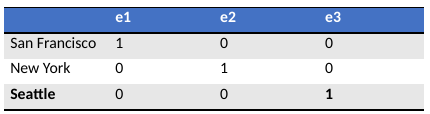
\includegraphics[scale=0.6]{images/Data
  pre-process/one hot encoding.png}
  \caption{Example of one-hot encoding}
  \label{fig:one-hot-encoding}
\end{figure}
Take a look at figure \ref{fig:one-hot-encoding} to see an example of 
one-hot encoding, as you can see the attribute city can only assume 3
values.

\subsubsection{Dummy Coding}
One-hot encoding allows for k degrees of freedom( where k is the
number of categories), but variable itself needs only k–1 degrees of 
freedom.\\
Dummy Coding encodes the effect of each category relative to the
reference category encoded with zeroes (Seattle).
\begin{figure}[H]
  \centering
  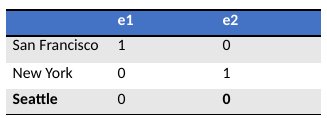
\includegraphics[scale=0.6]{images/Data
  pre-process/dummy coding.png}
  \caption{Example of dummy coding}
  \label{fig:dummy-coding}
\end{figure}

\subsubsection{Effect Coding}
Effect coding is similar to dummy coding, but the reference category 
is encoded with -1 instead of 0.\\ 
Effect coding is useful when you want to compare each category to the 
average of all categories.

\begin{figure}[H]
  \centering
  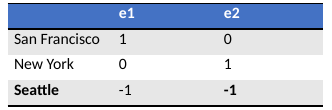
\includegraphics[scale=0.6]{images/Data
  pre-process/effect coding.png}
  \caption{Example of effect coding}
  \label{fig:effect-coding}
\end{figure}

\begin{figure}[H]
  \centering
  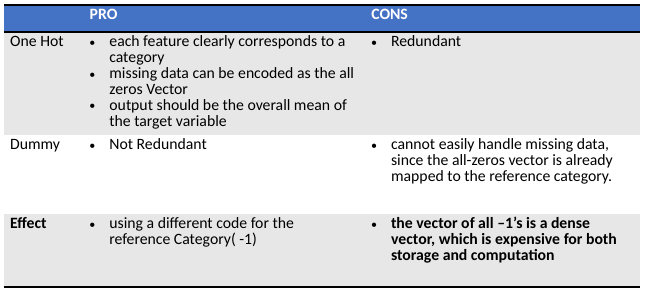
\includegraphics[scale=0.6]{images/Data
  pre-process/coding comparison.png}
  \caption{Comparison between dummy, effect and one-hot coding}
\end{figure}

\section{Attribute Transformation}
An \textbf{attribute transformation} is a mapping of the entire set of
values of a given attribute to a new set of replacement values such 
that each old value can be identified with one of the new values.\\ 
If can be a simple function like $x' = x^2$ or a more complex one like 
$ x' = \dfrac{x-\mu}{\sigma}$


\subsection{Normalization}

\textbf{Normalization} refers to various techniques to adjust to
differences among attributes in terms of mean, variance, range. It is
performed with the attribute transform that is is a function that maps
the entire set of values of a given attribute to a new set of
replacement values such that each old value can be identified with one
of the new values. There are a lot of different normalization.
\subsubsection{Min-Max normalization}
\begin{center}
    Min-max normalization  $x'= \dfrac{x-x_{min}}{x_{max} - x_{min}}$
\end{center}
Min Max-normalization rescales the functions and is a unity based
normalization, is a technique that bring all values into the range of
[0,1] retains the shape of the distribution, as shown in the figure 
\ref{fig:min-max-normalization}.
\begin{figure}[H]
    \centering
    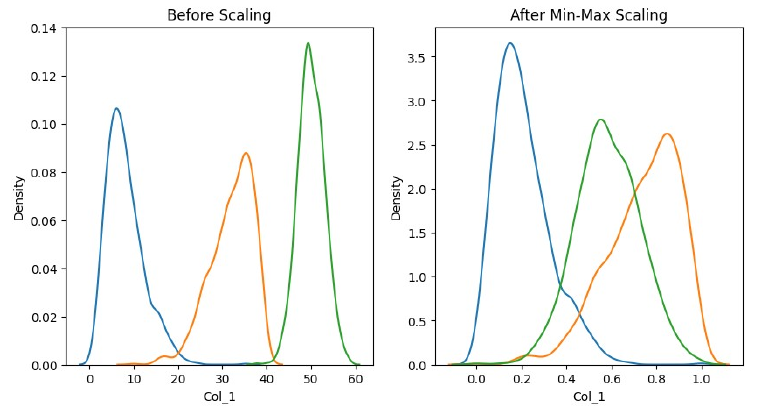
\includegraphics[scale=0.5]{images/Data pre-process/MINMAX.png}
    \caption{Example of Min max normalization}
    \label{fig:min-max-normalization}
\end{figure}
\subsubsection{Standardization}

\begin{center}
    Standardization  $x'= \dfrac{x- \mu}{\sigma}$
\end{center}

Standardization is another kind of normalization ans is a bit
different from the previous one because it is not bounded to a certain
range and it's used when we want to ensure zero mean and
unit standard deviation.
\begin{figure}[H]
    \centering
    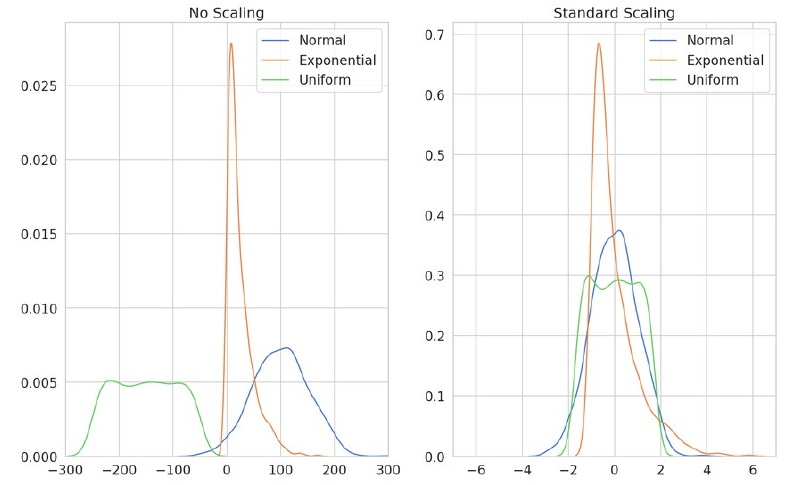
\includegraphics[scale=0.5]{images/Data pre-process/Standard.png}
    \caption{Example of standardization}
    \label{fig:enter-label}
\end{figure}

\section{Data preparation for document data}

Document may be modeled in different ways and the choice heavily
affects the quality of the mining result: often document are
represented as a set of features and might represent set of
characters, word, term, concept. 
\begin{boxH}
  Document preprocessing is the activity of generating a structured
  data representation of document data.
\end{boxH}
This includes 5 main steps:
\begin{enumerate}
    \item Document splitting
    \item Tokenization
    \item Case normalization
    \item Stopword removal
    \item Stemming
\end{enumerate}
\subsection{Document splitting}
Document splitting is based on the data analytics goal, documents can
be split into sentences, paragraphs, or analyzed in their entire
content.\\
Short documents are typically not split, like emails or social posts
but long documents can be split into paragraphs or sentences, or even
analyzed as a whole.
\subsection{Tokenization}
Tokenization is the process of breaking text into words, phrases, 
symbols or other meaningful elements.\\
To perform tokenization, one must first identify the boundaries of 
sentences based on punctuation and capitalization, and then split the 
text into words.
\subsection{Case normalization}
This step converts each token to completely upper-case or lower-case
characters.\\
Capitalisation helps human readers differentiate, for example, between
nouns and proper nouns and can be useful for automated algorithms as
well. However, an upper-case word at the beginning of the sentence
should be treated no differently than the same word in lower case
appearing elsewhere in a document.
\subsection{Stopword removal}
“Stop words” refers to the most common words in a language, for
example propositions, articles, and conjunctions.\\
Those are usually filtered out before or after processing of text,
because most likely they have little semantic meaning.
\section{Text representation}
Some algorithms can't process raw textual data directly, so documents
are converted into feature vectors for easier handling. A feature is a
simple entity, representing a dimension in the feature space, and a
document is represented as a vector of features with their
corresponding weights.
\subsection{Bag of words}

\textbf{Bag of words} are the representation for the words in a
document where every word is considered as a feature, where the
dimension is equal to the number of different words and there is a set
of weights, one for each distinct word.

\begin{figure}[H]
    \centering
    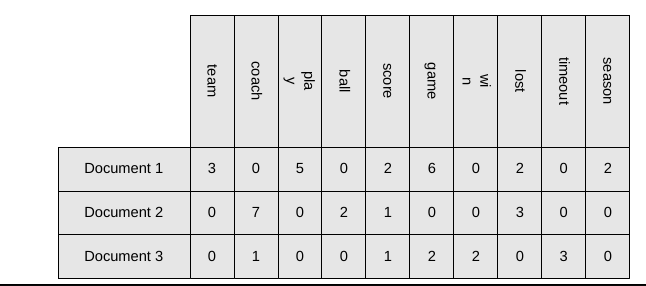
\includegraphics[scale=0.6]{images/Data pre-process/Word-bag.png}
    \caption{Example of bag of word}
    \label{fig:enter-label}
\end{figure}

\subsection{Weighting schemes}
Weighting schemes are used to assign weights to the words in the
document. They can be:
\begin{itemize}
    \item  Binary
        \begin{itemize}
            \item One, if the corresponding word is present in the document
            \item Zero, otherwise
            \item Occurrences of all words have the same importance
        \end{itemize}
    \item Simple document frequency
        \begin{itemize}
            \item The number of times in which the corresponding word occurs in the document
            \item Most frequent words are not always representative of the document content
        \end{itemize}
    \item Term frequency inverse document frequency (tf-idf)
        \begin{itemize}
            \item Tf-idf of term $t$ in document d of collection $D$ (consisting of m documents)
            \item Terms occurring frequently in a single document but rarely in the whole collection are preferred
            \item  tf-idf(t)$=   freq(t,d)\cdot log(\dfrac{m}{freq(t,D)} ) $
        \end{itemize}
\end{itemize}
Notice that the tf-idf is the most used weighting scheme because it 
gives more importance to the words that are more relevant to the 
document, and is also most suitable for a single document consisting
of many sections or subsections or a collection of documents.


 
